% MusicFormats CLI user guide
% Jacques Menu, 2021-2022

\documentclass[11pt,a4paper]{report}


% -------------------------------------------------------------------------
% import common LaTeX settings
% -------------------------------------------------------------------------

\usepackage{import}

\subimport{../CommonLaTeXFiles}{LaTeXCommonSettings.tex}

\subimport{../CommonLaTeXFiles}{LaTeXDivisionsCommands.tex}

\subimport{../CommonLaTeXFiles}{LaTeXIndexing.tex}

\subimport{../CommonLaTeXFiles}{LaTeXFontsAndColors.tex}

\subimport{../CommonLaTeXFiles}{LaTeXReferencing.tex}

\subimport{../CommonLaTeXFiles}{LaTeXBoxes.tex}

\subimport{../CommonLaTeXFiles}{LaTeXGraphicsAndPictures.tex}

\subimport{../CommonLaTeXFiles}{LaTeXMusicFormatsCommands.tex}

\subimport{../CommonLaTeXFiles}{LaTeXMusicFormatsFilesAndFolders.tex}

\subimport{../CommonLaTeXFiles}{LaTeXMusicFormatsNames.tex}

\subimport{../CommonLaTeXFiles}{LaTeXShortcuts.tex}

\subimport{../CommonLaTeXFiles}{LaTeXListings.tex}

\subimport{../CommonLaTeXFiles}{LaTeXTablesAndLists.tex}

\subimport{../CommonLaTeXFiles}{LaTeXMusicNotation.tex}


% -------------------------------------------------------------------------
% indexing (specific to this document)
% -------------------------------------------------------------------------

\makeindex[name=Main, options= -s ../CommonLaTeXFiles/MusicFormats.ist, columns=2, title=Main index, intoc]

% JMI don't create too many indexes, this causes idxlayout not to produce any indexes at all!

\makeindex[name=Files, options= -s ../CommonLaTeXFiles/MusicFormats.ist, columns=2, title=Files index, intoc]
%
%\makeindex[name=Types, options= -s ../CommonLaTeXFiles/MusicFormats.ist, columns=2, title=Types index, intoc]
%
%\makeindex[name=MethodsAndFields, options= -s ../CommonLaTeXFiles/MusicFormats.ist, columns=2, title=Methods and fields index, intoc]
%
%\makeindex[name=ConstantsFunctionsAndVariables, options= -s ../CommonLaTeXFiles/MusicFormats.ist, columns=2, title={Constants, functions and variables index}, intoc]
%
\makeindex[name=Options, options= -s ../CommonLaTeXFiles/MusicFormats.ist, columns=2, title=Options, intoc]
%
\makeindex[name=MusicXML, options= -s ../CommonLaTeXFiles/MusicFormats.ist, columns=2, title=MusicXML index, intoc]

\indexsetup{level=\section}


%\usepackage{cleveref}
	% http://tug.ctan.org/tex-archive/macros/latex/contrib/cleveref/cleveref.pdf


% -------------------------------------------------------------------------
\begin{document}
% -------------------------------------------------------------------------

% defeat headwidth not being equal to \textwidth %%%JMI should not be necessary ???
\setlength{\headwidth}{\textwidth}

% use the lists fancyhead headers and footers
\useListsPagesHeadersAndFooters


%%%JMI

%\makeatletter
%\let\Chapter@Original=\chapter
%\renewcommand{\chapter}{%
%	{%
%		\tiny%
%  	\Chapter@Original%
%	}%
%	\normalsize%
%}
%\makeatother

%\makeatletter
%\renewcommand \thepart {\@Roman\c@part}
%\renewcommand \thechapter {\@arabic\c@chapter}
%\renewcommand \thesection {\thechapter.\@arabic\c@section}
%\renewcommand\thesubsection   {\thesection.\@arabic\c@subsection}
%\renewcommand\thesubsubsection{\thesubsection .\@arabic\c@subsubsection}
%\renewcommand\theparagraph    {\thesubsubsection.\@arabic\c@paragraph}
%\renewcommand\thesubparagraph {\theparagraph.\@arabic\c@subparagraph}
%\makeatother


\begin{titlepage}
  \begin{center}
    \vspace*{2cm}

    \textbf{
      \LARGE{\mf\ user guide} \\[10pt]
			\Large{\url{https://github.com/jacques-menu/musicformats}}
		}

    \vspace{0.25cm}

    \large{
    	v\input{../../MusicFormatsVersionNumber.txt}%
			-- %
    	\input{../../MusicFormatsVersionDate.txt}
		}

    \vspace{0.75cm}

    \large{\textbf{Jacques Menu}}
  \end{center}

  \vspace{1cm}


\mf\ is open source software, available with source code and documentation at \url{https://github.com/jacques-menu/musicformats}. It is written in \CPlusplus\ and provides a set of music scores representations and converters between various textual music scores formats. Building it only requires a \CPlusplus\ compiler and \cmake.

This document shows how to use the \mf\ library, both from the \CLI\ and from within applications. It is part of the \mf\ documentation, and can be found at \gitdocpdf{MusicFormatsUserGuide}{MusicFormatsUserGuide.pdf}.

\mf\ can be used from the \CLI\ on Linux, Windows and Mac OS. The \API\ also allows it to be used from applications, including in \Web\ sites.


  \begin{center}
\begin{turn}{1}
\maxsizebox{0.9\linewidth}{5cm}{
\begin{minipage}{\linewidth}
\begin{lstlisting}[language=Terminal]
jacquesmenu@macmini > xml2ly -about
What xml2ly does:

    This multi-pass converter basically performs 5 passes:
        Pass 1:  reads the contents of MusicXMLFile or stdin ('-')
                 and converts it to a MusicXML tree;
        Pass 2a: converts that MusicXML tree into
                 a first Music Score Representation (MSR) skeleton;
        Pass 2b: populates the first MSR skeleton from the MusicXML tree
                 to get a full MSR;
        Pass 3:  converts the first MSR into a second MSR to apply options
        Pass 4:  converts the second MSR into a
                 LilyPond Score Representation (LPSR);
        Pass 5:  converts the LPSR to LilyPond code
                 and writes it to standard output.

    Other passes are performed according to the options, such as
    displaying views of the internal data or printing a summary of the score.

    The activity log and warning/error messages go to standard error.
}\end{lstlisting} % no line break here
\end{minipage}
}
\end{turn}

    \vspace{.5cm}

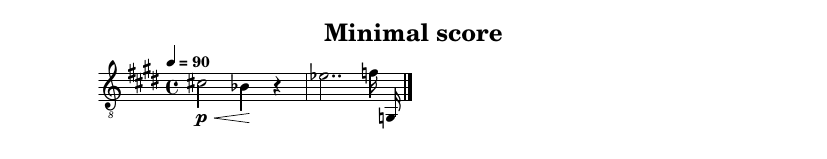
\includegraphics[scale=1.0]{../graphics/MinimalScore.png}

  \vfill

  \end{center}
\end{titlepage}

% -------------------------------------------------------------------------
{ % reduce vertical size of tables and lists
  \setlength {\parskip} {0.3ex plus \baselineskip minus 2pt}

  \tableofcontents

  \listoffigures
}


%% -------------------------------------------------------------------------
\part{Preamble}
%% -------------------------------------------------------------------------


% now we can switch to the regular headers and footers
\useRegularPagesHeadersAndFooters


\subimport{./}{acknowledgements}

\subimport{./}{about}


% -------------------------------------------------------------------------
\part{Discovering MusicFormats}
% -------------------------------------------------------------------------

\subimport{./}{architecture.tex}

\subimport{./}{aFirstExample.tex}

\subimport{./}{moreExamples.tex}

\subimport{./}{multipleFilesConversion.tex}

\subimport{./}{repository.tex}

\subimport{./}{libraryComponents.tex}

\subimport{./}{musicScoreView.tex}

\subimport{./}{versionsNumbering.tex}


% -------------------------------------------------------------------------
\part{Shell basics}
% -------------------------------------------------------------------------

\subimport{./}{shellBasics.tex}


% -------------------------------------------------------------------------
\part{Installing MusicFormats}
% -------------------------------------------------------------------------

\subimport{./}{installing.tex}


% -------------------------------------------------------------------------
\part{Options and help (OAH)}
% -------------------------------------------------------------------------

\subimport{./}{optionsAndHelp.tex}

\subimport{./}{nonMusicalOptions.tex}

\subimport{./}{traceOptions.tex}

%\subimport{./}{inputAndOutput}%%%JMI


% -------------------------------------------------------------------------
\part{Warnings and errors (WAE)}
% -------------------------------------------------------------------------

\subimport{./}{warningsAndErrors.tex}


% -------------------------------------------------------------------------
\part{Multiple languages support}
% -------------------------------------------------------------------------

\subimport{./}{multipleLanguagesSupport.tex}


% -------------------------------------------------------------------------
\part{The MusicFormats Scripting Language (MFSL)}
% -------------------------------------------------------------------------

\subimport{./}{theMFSLLanguage.tex}


% -------------------------------------------------------------------------
\part{{\tt xml2ly}}
% -------------------------------------------------------------------------

\subimport{./}{xml2ly.tex}


% -------------------------------------------------------------------------
\part{{\tt xml2brl}}
% -------------------------------------------------------------------------

\subimport{./}{xml2brl.tex}


% -------------------------------------------------------------------------
\part{{\tt xml2xml}}
% -------------------------------------------------------------------------

\subimport{./}{xml2xml.tex}


% -------------------------------------------------------------------------
\part{{\tt xml2gmn}}
% -------------------------------------------------------------------------

\subimport{./}{xml2gmn.tex}


% -------------------------------------------------------------------------
% postamble
% -------------------------------------------------------------------------

% -------------------------------------------------------------------------
\part{Indexes}
% -------------------------------------------------------------------------

% back to the lists fancyhead headers and footers
\useListsPagesHeadersAndFooters

\printindex[Files]

\printindex[Options]

\printindex[MusicXML]

\printindex[Main]


% -------------------------------------------------------------------------
\end{document}
% -------------------------------------------------------------------------
